\setlength{\parindent}{2em} %首行缩进

\section{實驗目的:}

\begin{enumerate}[label=\arabic*.]
  \item 透過 SDS-PAGE 電泳分析蛋白質分子量
\end{enumerate}

\section{實驗原理:}

\subsection{聚丙烯醯胺膠体電泳}
\begin{enumerate}
  \item 膠體成分
  \begin{enumerate}[label=\alph*.]
    \item 丙烯醯胺(acrylamide,單體分子)
    \begin{itemize}[]
      \item[-] 具有神經毒性,須戴手套、避免吸入。
      \item[-]  構成孔洞分離物質,acrylamide 濃度越高則孔洞越小。
    \end{itemize}

    \item Bis-acrylamide (架橋分子)
    \begin{itemize}[]
      \item[-] 可看作兩個丙烯醯胺單體分子連結,形成分叉點,幫助膠體聚合。
      \item[-] 和 Acrylamide 一樣具有神經毒性。
    \end{itemize}
    \item Ammonium persulfate(APS,自由基)
    \begin{itemize}[]
      \item[-] 產生自由基啟動膠體聚合反映。
    \end{itemize}
    \item Tetramethylethylenediamine(TEMED,催化劑)
    \begin{itemize}[]
      \item[-] 幫助自由基傳遞 
    \end{itemize}
  \end{enumerate}

  \begin{center}
    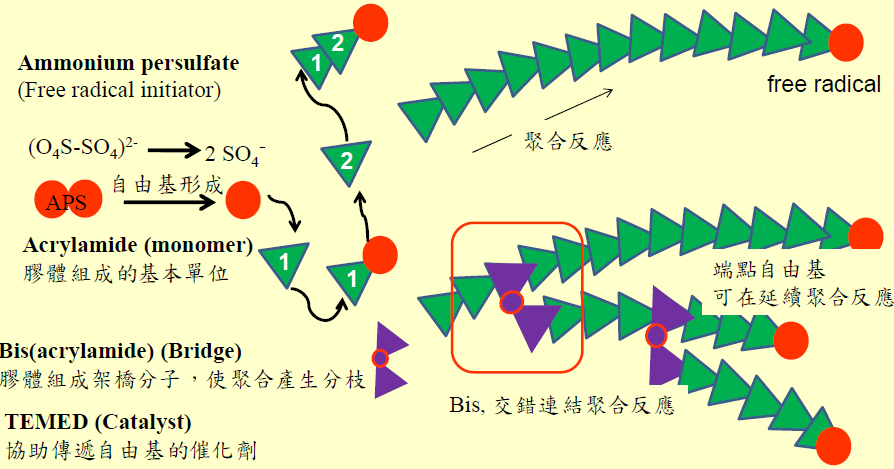
\includegraphics[width=.7\textwidth]{paste_src/2023-11-13-16-17-57.png}
  \end{center}

  \item 梯度電泳系統
  






  \begin{enumerate}[label=\alph*.]
    \item Stacking Gel 功能\\
    \hspace*{2em}Stacking gel 保證電泳時所有待測物在相同起跑點。樣品為鹼性環境(pH8.3),待測蛋白、Glycine 與 \ce{Cl^-} 都帶負電。Gly 的 pI 為 6.0,其在Stacking gel (pH6.9)中解離度較小。因此 Gly 在通電下移動緩慢,會阻礙待測蛋白前進。另外Stacking gel 的孔徑大,幾乎不會阻止蛋白質前進,最終待測蛋白會被壓在Stacking gel 邊界。
    \newpage
    \item 影響電泳泳動率的因素
    \begin{itemize}
      \item[-] 電場強度
      \item[-] 樣品電荷量
      \item[-] 樣品分子量
    \end{itemize}
  \end{enumerate}

  \begin{figure}[H]
    \begin{minipage}[h]{0.6\textwidth} %minipage寬
      \begin{tabular}{cccc}
        \toprule
        名稱  &pH &緩衝液&膠體濃度\\
        \midrule
        上層緩衝液(-) & 8.3 & Tris-glycine & - \\ 
        樣本 & 8.3 & Tris-glycine & -\\
        Stacking gel& 6.9& Tris-HCl & 低(約4\%)\\
        Separating gel& 8.3& Tris-HCl &高(約20\%)\\
        下層緩衝液(+) & 8.3& Tris-glycine & -\\
        \bottomrule
        \end{tabular}
    \end{minipage}
    \begin{minipage}[h]{0.35\textwidth} %minipage宽
    \centering
    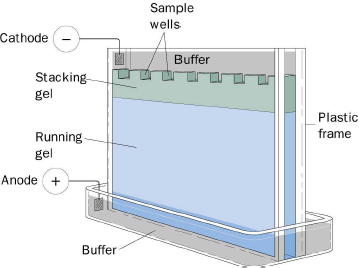
\includegraphics[width=1\textwidth]{paste_src/2023-11-13-16-00-45.png}
    \end{minipage}
  \end{figure}
\end{enumerate}


\subsection{SDS 及分子量測定}

Sodium dodecyl sulfate(SDS) 是界面活性劑,會在蛋白質分子表面均勻佈上一層負電荷,使得蛋白質電泳的結果不受馾白質自身電性影響。因此 SDS 電泳的結果只和蛋白質分子量相關。$\ce{\beta}$-mercaptoethanol(β-ME, 2-ME) 和 Dithiothreitol(DTT) 都能打斷雙硫鍵,同樣濃度下 DDT 效果較好。兩者會搭配 SDS 使用。

\subsection{蛋白質染色方法}

\begin{table}[ht]




\begin{tabular}{llll}
\toprule
染色方法 &染色對象 &靈敏度 &效果 \\
\midrule
Coomassie Brillant Blue R-250 &所有蛋白質 &中&簡單快速\\
Ammonical Silver &所有蛋白質(修飾後染醣) &高&較繁複\\
Periodic Acid-Schiff's Reagent(PAS) &所有糖類&低&非常繁複\\
紫外光吸收(300nm) &可吸收該波長蛋白質 &低&照射紫外光 \\
放射性物質偵測&含放射性標示分子 &高&放射物質 \\
KCl 沉澱&蛋白質上有 SDS 者 &低&簡單快速 \\
活性染色 &酵素反應後有沈澱 &高& 較繁複\\
\bottomrule
\end{tabular}\end{table}




\section{實驗步驟:}

\subsection{鑄膠}

\hspace*{-2em}實驗材料
\begin{enumerate}[label=\arabic*.]
  \item 藥品: Resolving gel、Stacking gel、APS(10\%)、TEMED
  \item 器材:透明鑄膠台、綠固定夾、綠齒梳、厚玻璃片、薄玻璃片、襯條、RO 水
\end{enumerate}
\newpage
\hspace*{-2em}步驟

\begin{enumerate}[label=\arabic*.]
  \item 於15ml離心管中分裝 5ml seperating gel mix 並置於冰上,再加入100\mul  10\% APS 與 10\mul TEMED,最後pipetting 3-5次。
  \item 將混好的 seperating gel mix 利用滴管小心加入事先準備好的鑄膠設備中,將溶液加至記號處,上層加入適量RO水壓平(約1ml)。室溫靜置15-20分鐘,待膠體聚集。
  \item 移除上方水層
  \item 於15ml離心管中分裝 2.5ml stacking gel mix  並置於冰上,再加入 50\mul  5\% APS 與 5\mul TEMED,最後pipetting 3-5次。
  \item 將混好的 stacking gel mix 利用滴管小心加入剛剛鑄好上層的膠上。
  \item 將 comb 小心放入鑄膠設備玻璃板間,避免氣泡形成。室溫靜置15-20分鐘,待膠體聚集。
  \item 最後將 gel 連同 comb 與 玻璃板取出。
\end{enumerate}



\subsection{電泳} 
\hspace*{-2em}實驗材料

\begin{enumerate}[label=\arabic*.]
  \item 藥品:Protein ladder(作為marker使用)、蛋白質樣品(先前實驗預留) 、SDS PAGE sample buffer、SDS PAGE running buffer、staining buffer(Coomassie Brillant Blue R-250)
  \item 器材:電泳槽、SDS-PAGE 膠、電源供應器、micropipette、塑膠盒子
\end{enumerate}

\hspace*{-2em}實驗步驟 

\begin{enumerate}[label=\arabic*.]
  \item 配置以下藥品,對照樣品為配置好的 3μg蛋白質加7μl的水
  \begin{table}[ht]
  \centering
  \begin{tabular}{cccc}
    \toprule
    編號&蛋白質樣品&dd\ce{H2O}&2x sample buffer\\
    \midrule
    對照樣品(S)&-&-&10\mul\\
    \ce{S_2}&2\mul&8\mul&10\mul\\
    \ce{S_4}&4\mul&6\mul&10\mul\\
    \ce{S_4}&6\mul&4\mul&10\mul\\
    \bottomrule
  \end{tabular}\end{table}

  \item 將配好的溶液於水浴5分鐘,打斷蛋白質雙硫鍵。
  \item 將SDS-PAGE 膠放入電泳槽,再注入 Portein ladder、對照樣品、\ce{S_2}、\ce{S_4}、\ce{S_6}
  \item 於電泳槽添加buffer。以168V電壓跑約50min,至traffic dye恰跑到凝膠下緣即可停止。
  \item 小心取下凝膠,以spacer切除上部stacking gel的部分。(可用Spacer沾水再輕輕撬開玻璃)
  \item 將剩下的resolving gel置於塑膠盒中,在水中浸泡並置於微波爐加熱,再搖晃,重複數次直到膠體褪色。(去除 SDS)
  \item 倒掉RO水,將staining buffer倒進塑膠盒中(約20-30ml),再搖擺直至染色。
  \item 使用大量的清水進行退染,直到可見清楚的蛋白色帶及近無色的背景為止。
\end{enumerate}


\section*{實驗結果及討論:}
\subsection*{結果}

\begin{enumerate}[label=\arabic*.]
  \item 從 \prettyref{fig:result} 對照 marker 可看出所有樣品的分子量都約為 67
  \item 從 \prettyref{fig:result}可看出相較於對照樣品 S,\ce{S4}與 \ce{S6} 的藍色體積較大,顏色深度都較深更多;而 \ce{S2}則顏色較淺。
\end{enumerate}

\begin{figure}[H]
\centering
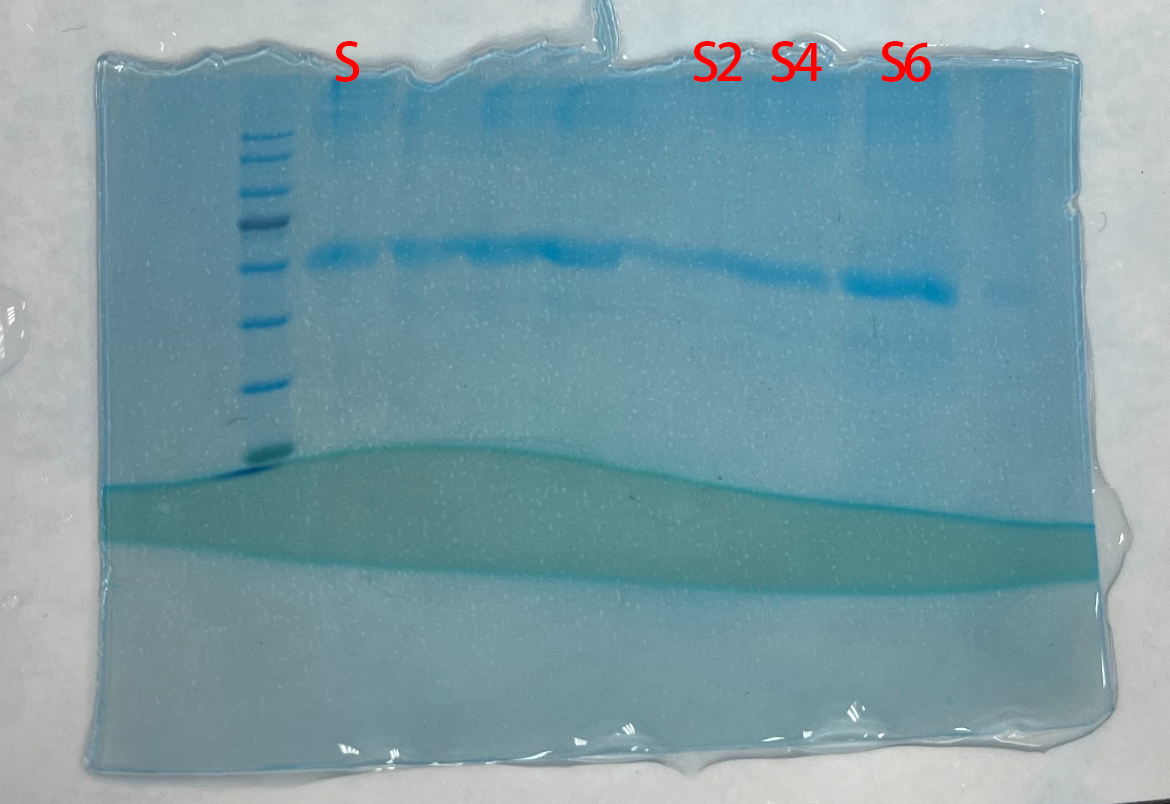
\includegraphics[width=0.8\textwidth]{paste_src/result.png}
\caption{電泳結果}
\label{fig:result}
\end{figure}



\newpage
\subsection*{實驗討論:}

\dsc 第二周準備進行電泳時,發現我們第一周的膠只有Separating gel而沒有Stacking gel?

推測可能是我們這組第一周進行膠片製備的時候,在膠片還沒有完全凝結的時候,就將其從鑄膠設備取下,導致Stacking gel流掉。

老師在上課有提到,在製備Stacking gel mix時,可以將其中冰上取下,如此就可以透過觀察Stacking gel mix,來判斷膠片是否已經凝結,然而我們等待許久,發現Stacking gel mix仍未有凝結的現象,於是拿著鑄膠設備,在助教認可凝結後將其取下。

膠體不凝結可能的原因有APS, TEMED, acrylamide等試劑的品質、室溫太低、膠體溶液的比例不對、APS濃度不夠等,我們覺得可能是APS濃度不夠,APS是自由基的產生者,負責將負電荷傳給Acrylamide,使其單體的電性改變,而去攻擊下一個單體,而若是濃度不夠,將使Acrylamide單體之間不結合,無法形成膠體。另外,老師也有提到膠體的比例改變,將使膠體凝結的時間增長,這也是可能的原因。 


\dsc 染料線歪斜的原因?

電泳的時候,我們逐漸發現染料線是歪的(\prettyref{fig:歪斜的染料線}),幸好助教經過,提醒我們是上方的緩衝液滲漏所導致,帶負電的蛋白質需要在通電的情況下才會移動,而左側上方的緩衝液滲漏,導致左側的蛋白質在沒有通電的情況下就不動了。後來,我們聽從助教的指示,隨時補充緩衝液,染料線歪斜的情形才逐漸消失。

\begin{figure}[H]
\centering
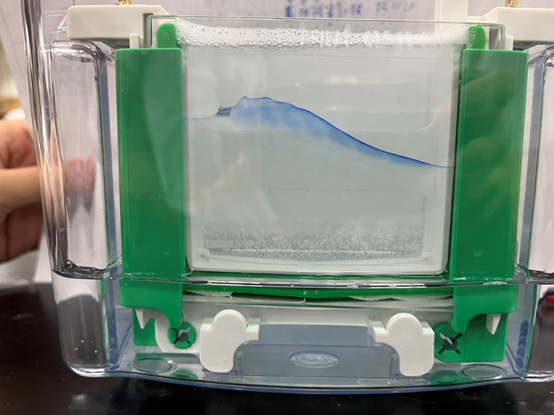
\includegraphics[width=.6\textwidth]{paste_src/2023-11-13-22-36-02.png}
\caption{歪斜的染料線}
\label{fig:歪斜的染料線}
\end{figure}




\newpage
\dsc 為什麼分離膠體區段之緩衝液pH值要8.3?

在PAGE系統當中,在分離膠體區段的緩衝液pH值使用8.3是因為大多數蛋白質等電點小於8.3,於是在這樣的pH值環境中,等電點小於8.3的蛋白質能夠順利地由上(-)往下(+)跑,反之,等電點大於或是等於8.3的蛋白質則不能夠順利游動。

而今天我們實驗因為添加了SDS,除了將蛋白質變性之外,又在蛋白質表面布上負電荷,這樣就不會受到pH值影響,都會由上往下跑,不過由於緩衝液使用的是tris-glycine,所以分離膠體區段緩衝液pH值8.3也能使glycine不要擋住我們要分離的蛋白質。\cite{3電泳62:online}
%參考資料:http://juang.bst.ntu.edu.tw/ECX/Ana3.htm


\dsc 老師提到「SDS-PAGE 可用來測定變性狀態 (denatured) 蛋白質 之 分子量,與原態 (native) 分子量可能不一樣。」有甚麼例子嗎?

由生化正課所學,我們已知蛋白質有一到四級結構,四級結構蛋白質由數個相同或不相同的三級結構分子組合成的蛋白質複合體,而這每一單位的分子又可稱為次體,次體與次體之間的鍵結為二級鍵(氫鍵)。所以加入SDS後,有可能會使四元體(假設其kDa為200)被分解為單元體(kDa為50),於是跑膠後能看到分子量更小的band,也就是發生與原態分子量不同的狀況。\cite{蛋白質17:online}
%參考資料:http://juang.bst.ntu.edu.tw/BC2008/Protein.htm#1.4


\dsc 電泳的電壓、電流與電阻

粒子移動速率與電壓梯度相關,一般使用 20-200 V/cm。使用較高的電壓可以更快得到結果,但精細度較差,也可能會導致電泳液過熱。

電泳的電阻只受緩衝液影響,然而電泳過程會產熱導致電泳液升溫而電阻下降。固定電壓下會導致電流增加,且使電泳液蒸發,因而破壞電泳結果的可重複性。\cite{v:online}



\bibliography{bibfile} 
\bibliographystyle{unsrt}
